\documentclass[a4paper,12pt,headsepline]{scrartcl} % Using KOMA-Script for better typography
\usepackage[utf8]{inputenc}
\usepackage{graphicx}
\usepackage{amsmath}
\usepackage{geometry}
\usepackage{hyperref}
\usepackage{booktabs}
\usepackage{fancyhdr}
\usepackage{times} % Using Times font for a classic look
\usepackage{xcolor}
\usepackage{caption}
\usepackage{listings}
\usepackage{tikz} % For advanced title page design
\usepackage{array} % For better table column control
\usepackage{float} % For better figure placement

% --- Professional Color & Style Definitions ---
\definecolor{IITJBlue}{RGB}{0, 51, 102}      
\definecolor{TextGray}{RGB}{45, 45, 45}     
\definecolor{HyperlinkBlue}{RGB}{0, 80, 155} 
\definecolor{CodeBackground}{RGB}{245, 245, 245}
\definecolor{CodeGray}{RGB}{128, 128, 128}

\hypersetup{
    colorlinks=true, linkcolor=HyperlinkBlue, filecolor=HyperlinkBlue,      
    urlcolor=HyperlinkBlue, citecolor=HyperlinkBlue
}

\geometry{margin=1in}
\color{TextGray}
\setkomafont{section}{\large\bfseries\color{IITJBlue}}
\setkomafont{subsection}{\bfseries\color{IITJBlue}}

% --- Python Code Block Styling ---
\lstdefinestyle{mystyle}{
    backgroundcolor=\color{CodeBackground},   
    commentstyle=\color{CodeGray}\itshape,
    keywordstyle=\color{IITJBlue},
    numberstyle=\tiny\color{CodeGray},
    stringstyle=\color{HyperlinkBlue},
    basicstyle=\footnotesize\ttfamily,
    breakatwhitespace=false, breaklines=true, captionpos=b, keepspaces=true,                 
    numbers=left, numbersep=5pt, showspaces=false, showstringspaces=false,
    showtabs=false, tabsize=2
}
\lstset{style=mystyle}

% --- Header and Footer Setup ---
\pagestyle{fancy}
\fancyhf{}
\fancyhead[L]{\textcolor{IITJBlue}{\small Machine Learning in Economics}}
\fancyhead[R]{\textcolor{IITJBlue}{\small Anushk Gupta, AIL 7310}}
\fancyfoot[C]{\thepage}
\renewcommand{\headrulewidth}{0.4pt}

\begin{document}

% --- Professional Title Page ---
\begin{titlepage}
    \centering
    \vspace*{2cm} % Add vertical space at the top
    
    % Placeholder for course logo (uncomment if logo file is available)
    % \includegraphics[width=0.5\textwidth]{cv_logo.png}
    
    \vspace{1cm} % Add space after logo (or top space if no logo)
    
    {\huge\color{IITJBlue} Machine Learning in Economics}
    
    \vspace{0.5cm}
    
    {\Large\itshape Assignment 02}
    
    \vfill % Pushes the content below to the bottom
    
    {\large\bfseries Anushk Gupta} \\
    {\mdseries AIL 7310}
    
    \vspace{0.8cm}
    
    {\large \href{https://github.com/introspective321/Sem_7_assignments}{\color{HyperlinkBlue}Link to GitHub Repository}}
    
    \vspace{1.5cm}
    
    {\large \today}
    
\end{titlepage}

\tableofcontents
\newpage

\section{Abstract}
This report presents a comprehensive analysis of causal inference methods applied to economic data. The study implements two major econometric techniques: Difference-in-Difference (DiD) analysis to estimate the causal impact of government subsidies on regional wages, and Regression Discontinuity Design (RDD) to evaluate the effect of scholarships on student test scores. The DiD analysis reveals a statistically significant positive treatment effect of \$1.68--\$1.79 on average wages (p < 0.001), with heterogeneous effects across sectors. The RDD analysis shows no significant effect in the full sample (p = 0.69) but demonstrates a large local effect of 6.13 points (p < 0.001) near the cutoff.

\section{Introduction}
Causal inference is fundamental to understanding policy impacts in economics. This report explores two widely-used quasi-experimental methods:

\begin{enumerate}
    \item \textbf{Difference-in-Difference (DiD)}: Exploits variation in treatment timing across groups to estimate causal effects, assuming parallel trends in the absence of treatment.
    \item \textbf{Regression Discontinuity Design (RDD)}: Leverages discontinuous treatment assignment based on a running variable to identify local treatment effects at the cutoff.
\end{enumerate}

The analysis uses real-world datasets: \texttt{did\_data.csv} containing information on 200 economic regions over 10 years (2006--2015), and \texttt{rdd\_data.csv} with data on 4,000 students and their test performance.

\section{Data Description}

\subsection{Difference-in-Difference Dataset}
The \texttt{did\_data.csv} dataset contains 2,000 observations with the following variables:
\begin{itemize}
    \item \textbf{region\_id}: Unique identifier for each economic region (200 regions)
    \item \textbf{sector}: Economic sector (Agriculture, Manufacturing, Services)
    \item \textbf{year}: Year of observation (2006--2015)
    \item \textbf{treatment}: Binary indicator for receiving government subsidy
    \item \textbf{population}: Regional population
    \item \textbf{unemployment\_rate}: Unemployment rate
    \item \textbf{gdp\_per\_capita}: GDP per capita
    \item \textbf{exports\_per\_capita}: Exports per capita
    \item \textbf{fdi\_inflow}: Foreign direct investment inflow
    \item \textbf{avg\_wage}: Average wage (outcome variable)
\end{itemize}

The treatment (subsidy) begins in 2010 for treated regions, creating a natural experiment with 100 treated and 100 control regions.

\subsection{Regression Discontinuity Dataset}
The \texttt{rdd\_data.csv} dataset contains 4,000 student observations with:
\begin{itemize}
    \item \textbf{student\_id}: Unique identifier
    \item \textbf{5th\_score}: Normalized 5th grade test score (running variable)
    \item \textbf{10th\_score}: 10th grade test score (outcome variable)
    \item \textbf{hours\_studied}: Hours studied per week
    \item \textbf{mother\_edu}: Mother's education (years)
    \item \textbf{female}: Gender indicator (1 = female, 0 = male)
\end{itemize}

Students with \texttt{5th\_score} > 0 receive scholarships, creating a sharp discontinuity at the cutoff.

\section{Methodology}

\subsection{Difference-in-Difference Analysis}

The DiD methodology involves the following steps:

\paragraph{a) Treated Variable Construction}
A binary variable \texttt{treated} was created to identify regions that ever receive treatment:
\begin{equation}
\text{treated}_i = \max_{t} \text{treatment}_{it}
\end{equation}

\paragraph{b) Post Variable Construction}
A binary variable \texttt{post} identifies the post-treatment period:
\begin{equation}
\text{post}_t = 
\begin{cases}
1 & \text{if } t \geq 2010 \\
0 & \text{if } t < 2010
\end{cases}
\end{equation}

\paragraph{c) Parallel Trends Assessment}
Visual inspection of pre-treatment trends (2006--2009) tests the parallel trends assumption.

\paragraph{d) Basic DiD Regression}
The basic DiD model is estimated using OLS:
\begin{equation}
\text{avg\_wage}_{it} = \beta_0 + \beta_1 \text{treated}_i + \beta_2 \text{post}_t + \beta_3 (\text{treated}_i \times \text{post}_t) + \epsilon_{it}
\end{equation}
where $\beta_3$ is the DiD estimator (treatment effect).

\paragraph{e) DiD with Control Variables}
The extended model includes confounders:
\begin{multline}
\text{avg\_wage}_{it} = \beta_0 + \beta_1 \text{treated}_i + \beta_2 \text{post}_t + \beta_3 (\text{treated}_i \times \text{post}_t) \\
+ \beta_4 \text{population}_{it} + \beta_5 \text{unemployment\_rate}_{it} + \beta_6 \text{gdp\_per\_capita}_{it} \\
+ \beta_7 \text{exports\_per\_capita}_{it} + \beta_8 \text{fdi\_inflow}_{it} + \epsilon_{it}
\end{multline}

\paragraph{f) Heterogeneous Treatment Effects}
Separate DiD regressions were estimated for each sector (Agriculture, Manufacturing, Services).

\subsection{Regression Discontinuity Design}

The RDD methodology includes:

\paragraph{a) Treatment Variable}
Binary treatment indicator based on the cutoff rule:
\begin{equation}
D_i = 
\begin{cases}
1 & \text{if } \text{5th\_score}_i > 0 \\
0 & \text{if } \text{5th\_score}_i \leq 0
\end{cases}
\end{equation}

\paragraph{b) Continuity Tests}
T-tests assess whether covariates (\texttt{hours\_studied}, \texttt{mother\_edu}) are continuous at the cutoff to detect potential manipulation.

\paragraph{c) Discontinuity Visualization}
Scatter plots and bin averages illustrate the jump in outcomes at the cutoff.

\paragraph{d) RDD Estimation}
Three models were estimated:

\textbf{Model 1: Basic RDD}
\begin{equation}
\text{10th\_score}_i = \alpha + \tau D_i + \beta X_i + \epsilon_i
\end{equation}
where $X_i = \text{5th\_score}_i$ (centered at cutoff).

\textbf{Model 2: RDD with Interaction}
\begin{equation}
\text{10th\_score}_i = \alpha + \tau D_i + \beta_1 X_i + \beta_2 (D_i \times X_i) + \epsilon_i
\end{equation}
allowing different slopes on each side of the cutoff.

\textbf{Model 3: Full Model with Covariates}
\begin{multline}
\text{10th\_score}_i = \alpha + \tau D_i + \beta_1 X_i + \beta_2 (D_i \times X_i) \\
+ \gamma_1 \text{hours\_studied}_i + \gamma_2 \text{mother\_edu}_i + \gamma_3 \text{female}_i + \epsilon_i
\end{multline}

\textbf{Robustness Check}
Local linear regression with bandwidth = 0.5 restricts analysis to observations near the cutoff.

\section{Results}

\subsection{Difference-in-Difference Analysis}

\subsubsection{Parallel Trends}
Figure \ref{fig:parallel_trends} shows the evolution of average wages over time for treated and control regions. The pre-treatment period (2006--2009) exhibits reasonably parallel trends, supporting the identifying assumption. After treatment begins in 2010, the treated group shows a steeper increase in wages compared to the control group.

\begin{figure}[H]
    \centering
    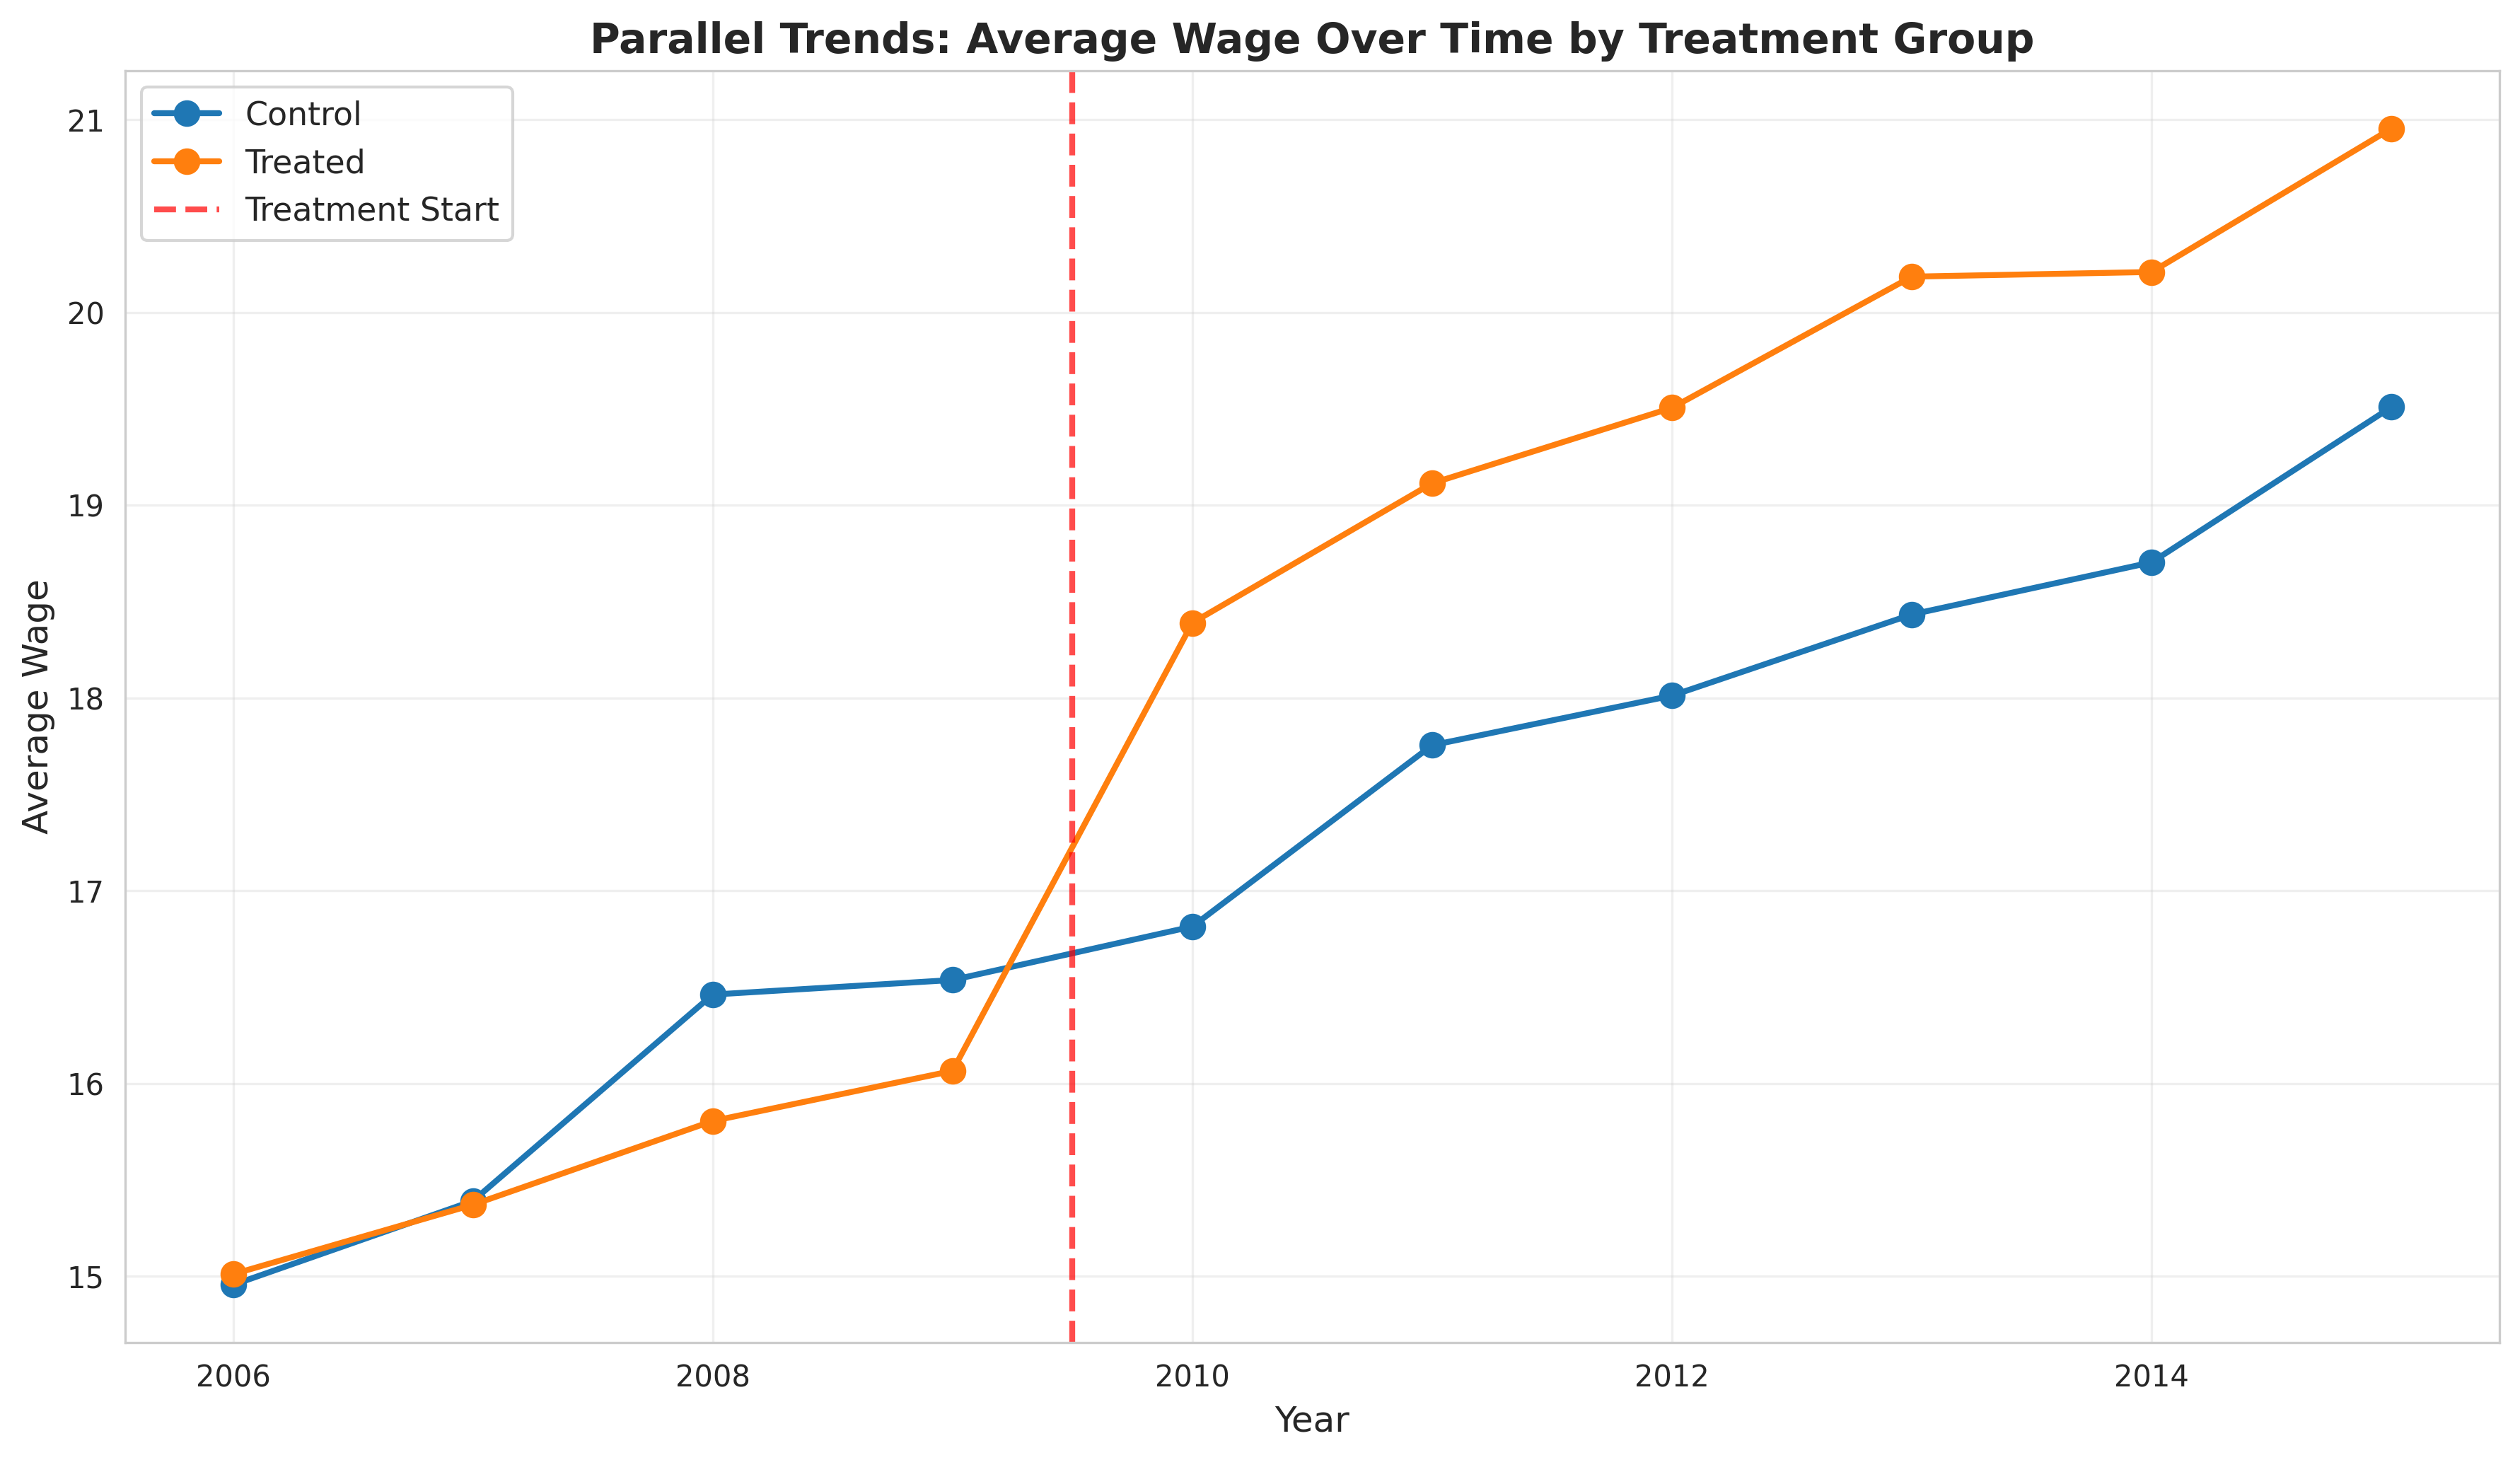
\includegraphics[width=0.85\textwidth]{parallel_trends_plot.png}
    \caption{Parallel trends: Average wage over time by treatment group. The vertical dashed line indicates the start of treatment in 2010. Pre-treatment trends appear approximately parallel, validating the DiD approach.}
    \label{fig:parallel_trends}
\end{figure}

\subsubsection{DiD Regression Results}

\textbf{Basic DiD Model:}
The basic DiD regression yields the following results:

\begin{table}[H]
\centering
\begin{tabular}{lcccc}
\toprule
Variable & Coefficient & Std. Error & t-statistic & p-value \\
\midrule
Intercept & 15.836 & 0.103 & 153.81 & <0.001 \\
treated & -0.273 & 0.146 & -1.87 & 0.061 \\
post & 2.368 & 0.133 & 17.82 & <0.001 \\
treated $\times$ post & \textbf{1.794} & 0.188 & 9.55 & <0.001 \\
\midrule
R-squared & \multicolumn{4}{c}{0.408} \\
\bottomrule
\end{tabular}
\caption{Basic DiD regression results. The treatment effect ($\beta_3$) is 1.794, indicating a \$1.79 increase in average wages due to the subsidy.}
\label{tab:did_basic}
\end{table}

\textbf{DiD with Control Variables:}
Adding control variables yields:

\begin{table}[H]
\centering
\small
\begin{tabular}{lcccc}
\toprule
Variable & Coefficient & Std. Error & t-statistic & p-value \\
\midrule
Intercept & 12.789 & 0.720 & 17.77 & <0.001 \\
treated & -0.226 & 0.146 & -1.54 & 0.123 \\
post & 2.173 & 0.141 & 15.44 & <0.001 \\
treated $\times$ post & \textbf{1.683} & 0.194 & 8.67 & <0.001 \\
population & $1.34 \times 10^{-5}$ & $5.73 \times 10^{-6}$ & 2.33 & 0.020 \\
unemployment\_rate & 5.741 & 2.317 & 2.48 & 0.013 \\
gdp\_per\_capita & $7.29 \times 10^{-5}$ & $3.94 \times 10^{-5}$ & 1.85 & 0.065 \\
\midrule
R-squared & \multicolumn{4}{c}{0.414} \\
\bottomrule
\end{tabular}
\caption{DiD regression with control variables. The treatment effect remains significant at \$1.68, with slight attenuation after controlling for confounders.}
\label{tab:did_controls}
\end{table}

\textbf{Interpretation:}
The government subsidy increases average wages by approximately \$1.68--\$1.79, depending on model specification. This effect is highly statistically significant (p < 0.001) and robust to the inclusion of control variables.

\subsubsection{Heterogeneous Treatment Effects}

The treatment effect varies substantially across sectors, as shown in Figure \ref{fig:heterogeneous} and Table \ref{tab:heterogeneous}.

\begin{figure}[H]
    \centering
    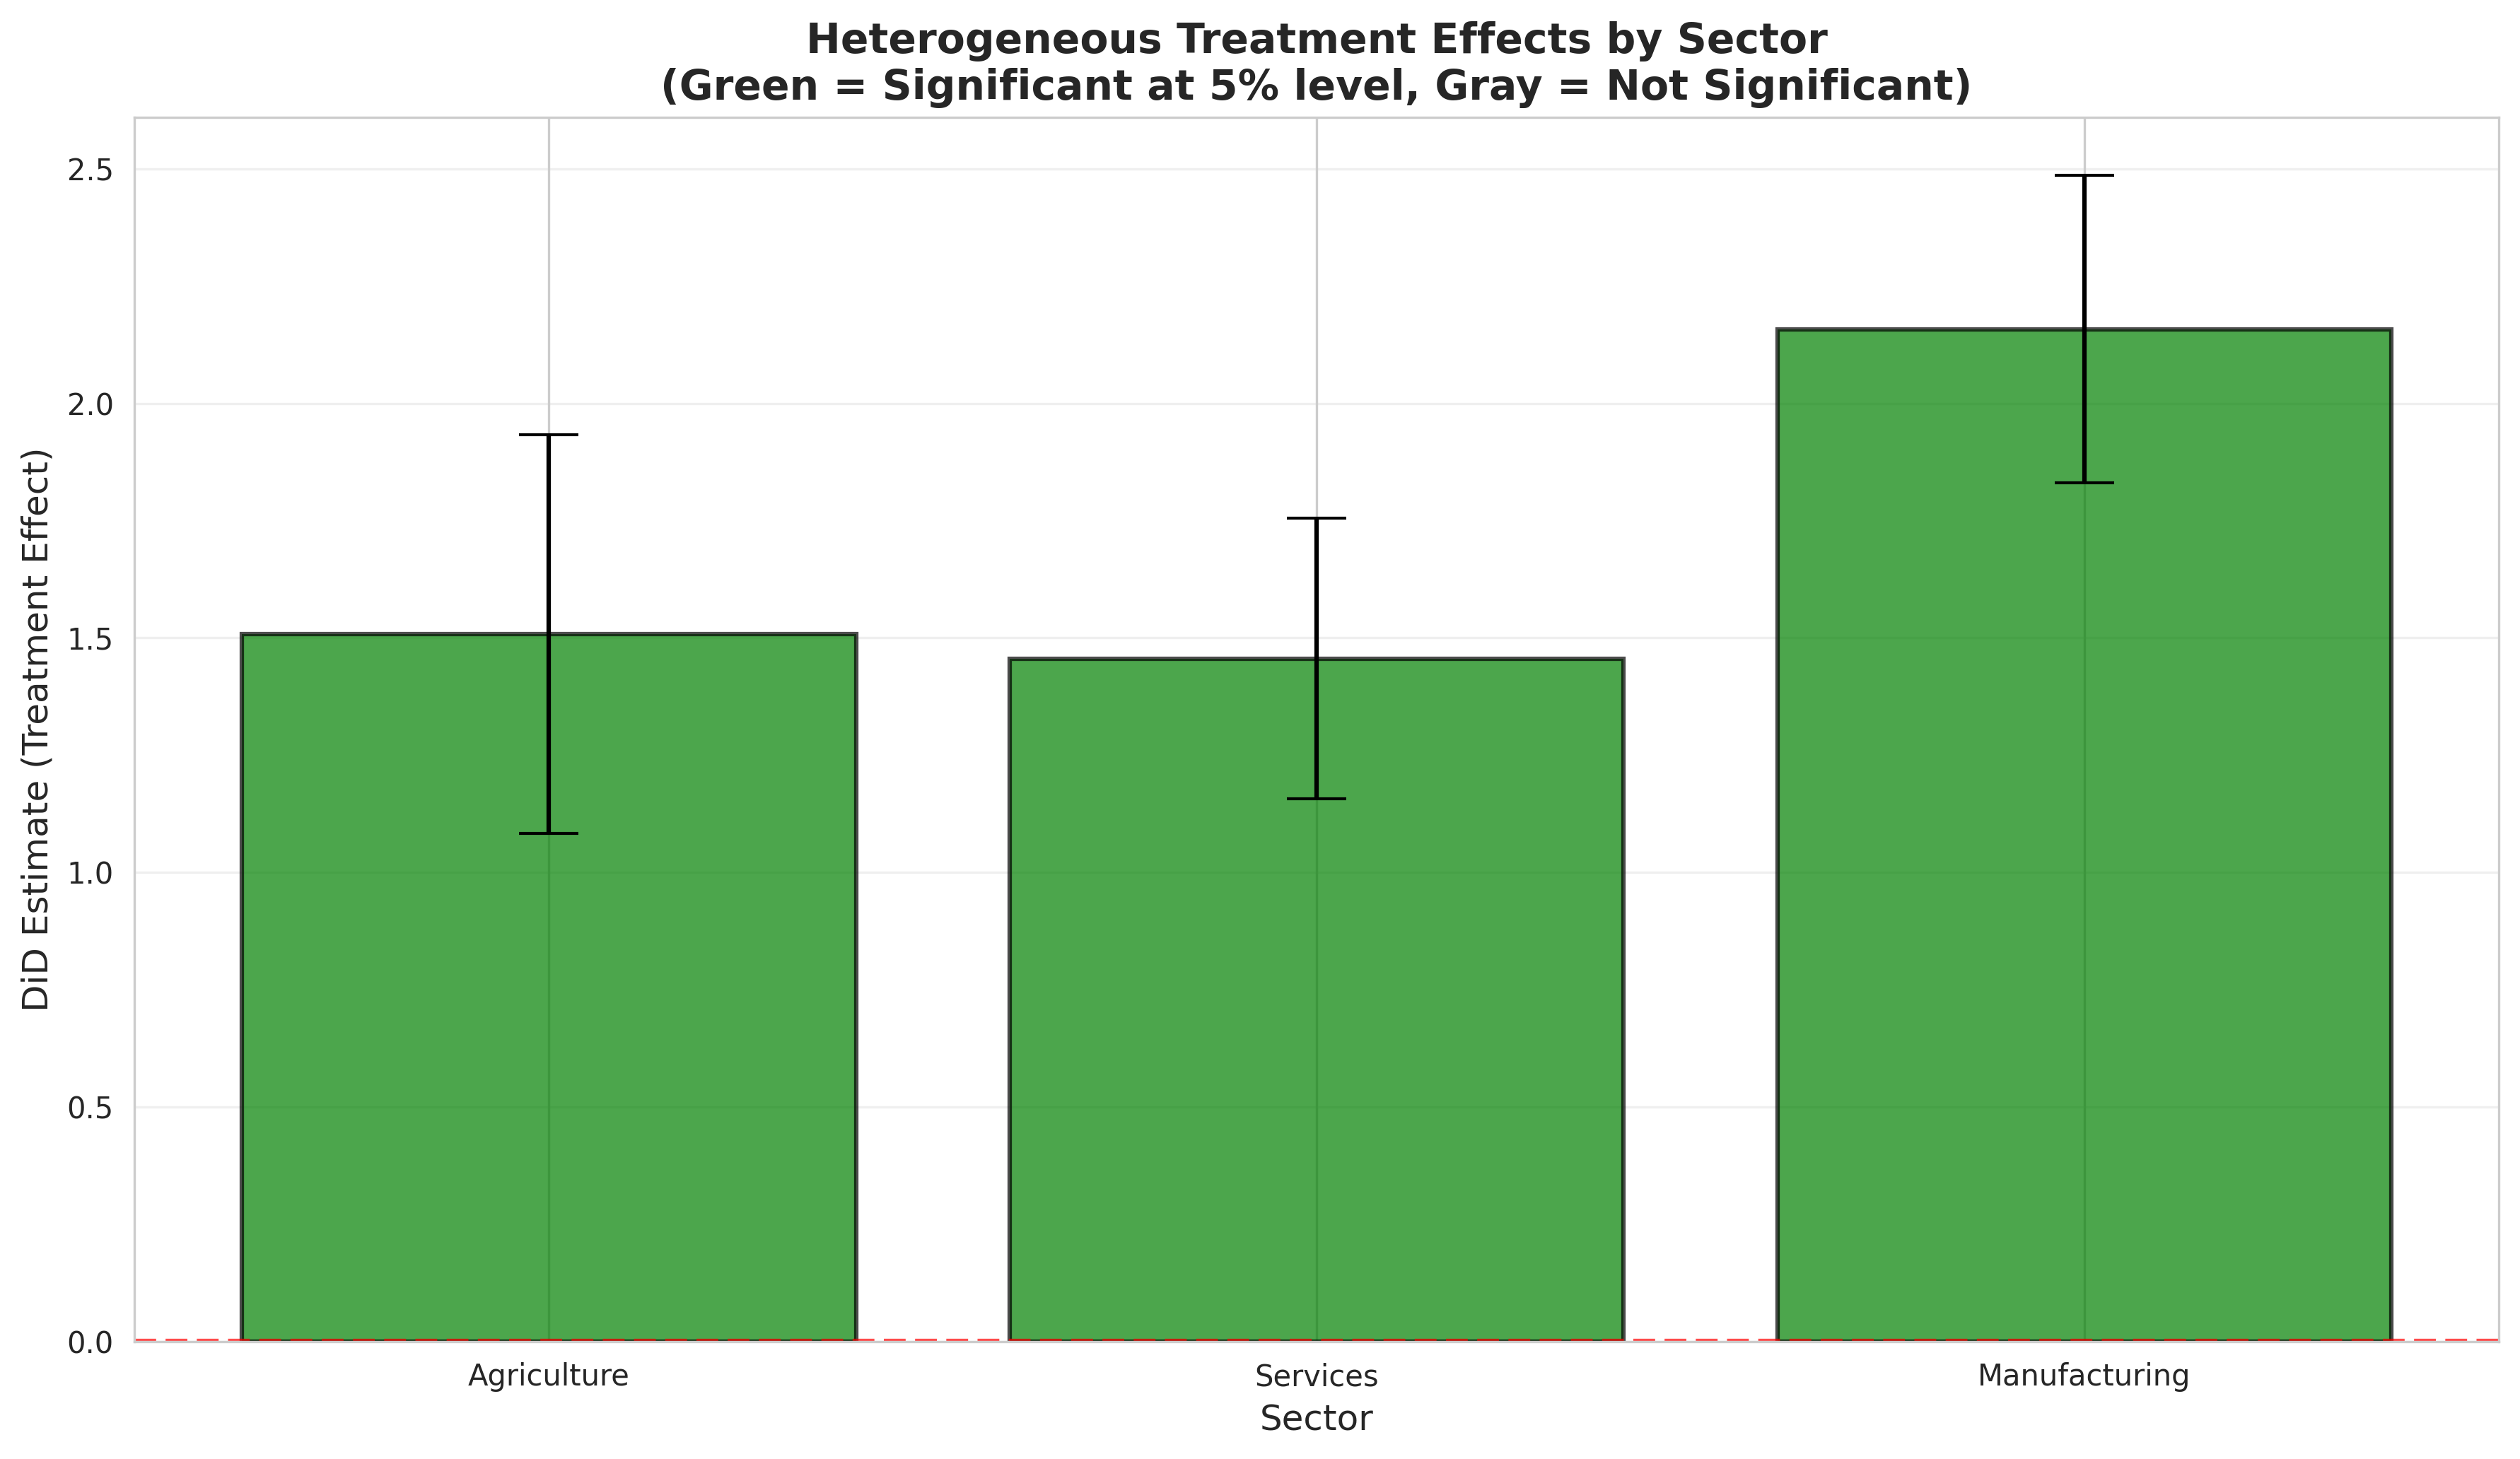
\includegraphics[width=0.85\textwidth]{heterogeneous_effects_plot.png}
    \caption{Heterogeneous treatment effects by sector. All three sectors show statistically significant positive effects (green bars), with Manufacturing experiencing the largest impact.}
    \label{fig:heterogeneous}
\end{figure}

\begin{table}[H]
\centering
\begin{tabular}{lcccc}
\toprule
Sector & DiD Estimate & Std. Error & p-value & Significant \\
\midrule
Manufacturing & \textbf{2.158} & 0.327 & <0.001 & Yes \\
Agriculture & 1.509 & 0.425 & <0.001 & Yes \\
Services & 1.456 & 0.299 & <0.001 & Yes \\
\bottomrule
\end{tabular}
\caption{Heterogeneous treatment effects by sector. Manufacturing experiences the largest wage increase (+\$2.16), while Services shows the smallest effect (+\$1.46).}
\label{tab:heterogeneous}
\end{table}

\textbf{Key Findings:}
\begin{itemize}
    \item All three sectors show statistically significant positive effects
    \item Manufacturing benefits most from the subsidy (+\$2.16)
    \item Services benefits least (+\$1.46)
    \item The range of treatment effects is \$0.70
\end{itemize}

\subsection{Regression Discontinuity Design}

\subsubsection{Continuity Tests}

Figure \ref{fig:continuity} displays continuity tests for covariates at the cutoff. Ideally, covariates should be continuous (no jump) at the threshold if there is no manipulation of the running variable.

\begin{figure}[H]
    \centering
    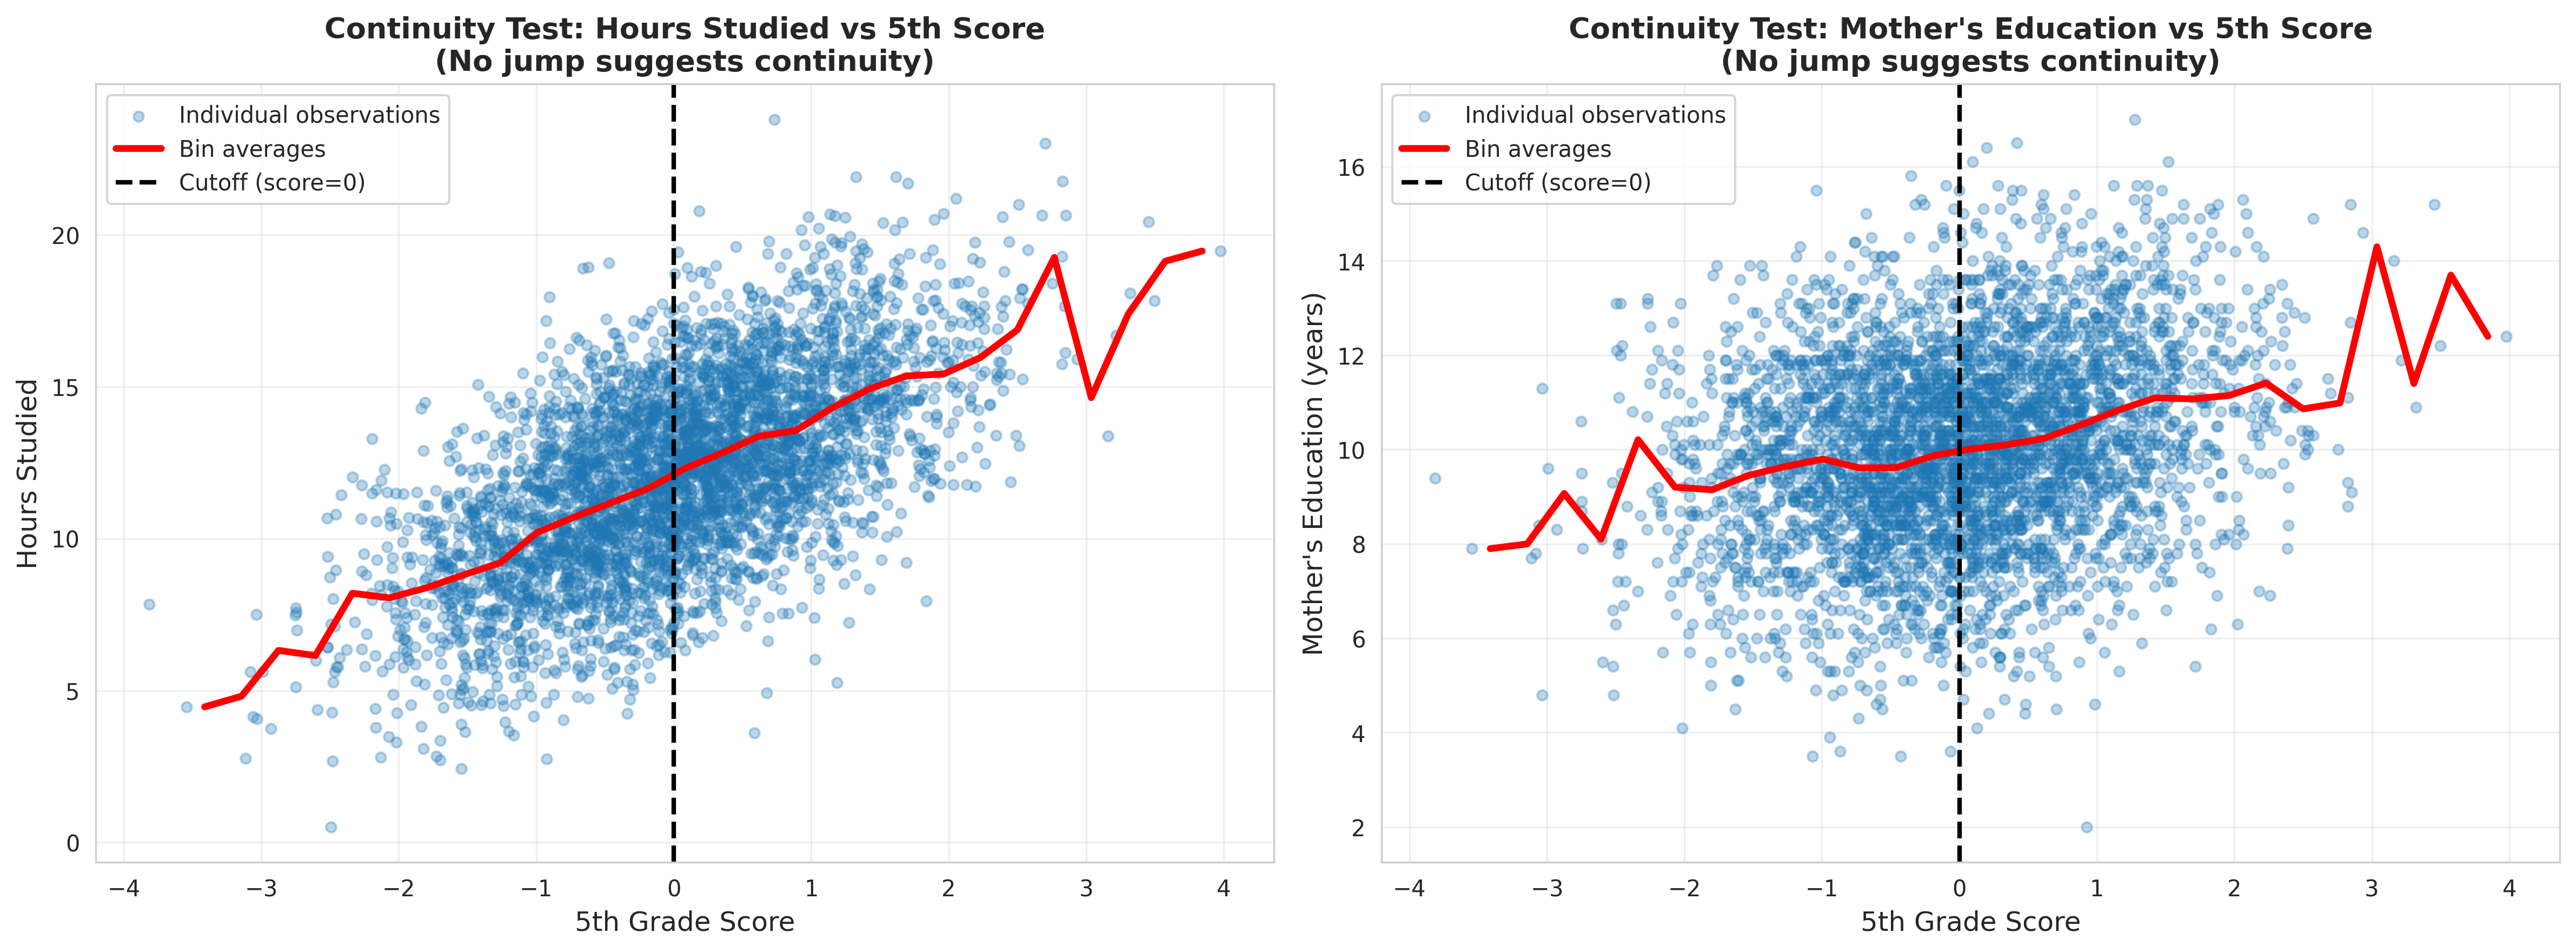
\includegraphics[width=\textwidth]{continuity_test_plot.png}
    \caption{Continuity tests for \texttt{hours\_studied} (left) and \texttt{mother\_edu} (right). Both show statistically significant discontinuities at the cutoff, suggesting potential manipulation or selection.}
    \label{fig:continuity}
\end{figure}

\textbf{Continuity Test Results:}
\begin{itemize}
    \item \textbf{Hours Studied}: Mean below cutoff = 11.52, mean above = 12.65, p-value < 0.001 (significant)
    \item \textbf{Mother's Education}: Mean below cutoff = 9.79 years, mean above = 10.09 years, p-value = 0.004 (significant)
\end{itemize}

⚠️ \textbf{Warning:} The significant discontinuities in covariates suggest potential violation of RDD assumptions through manipulation or selection at the cutoff.

\subsubsection{Discontinuity Visualization}

Figure \ref{fig:rdd_discontinuity} shows the relationship between 5th and 10th grade scores, with a visible jump at the cutoff.

\begin{figure}[H]
    \centering
    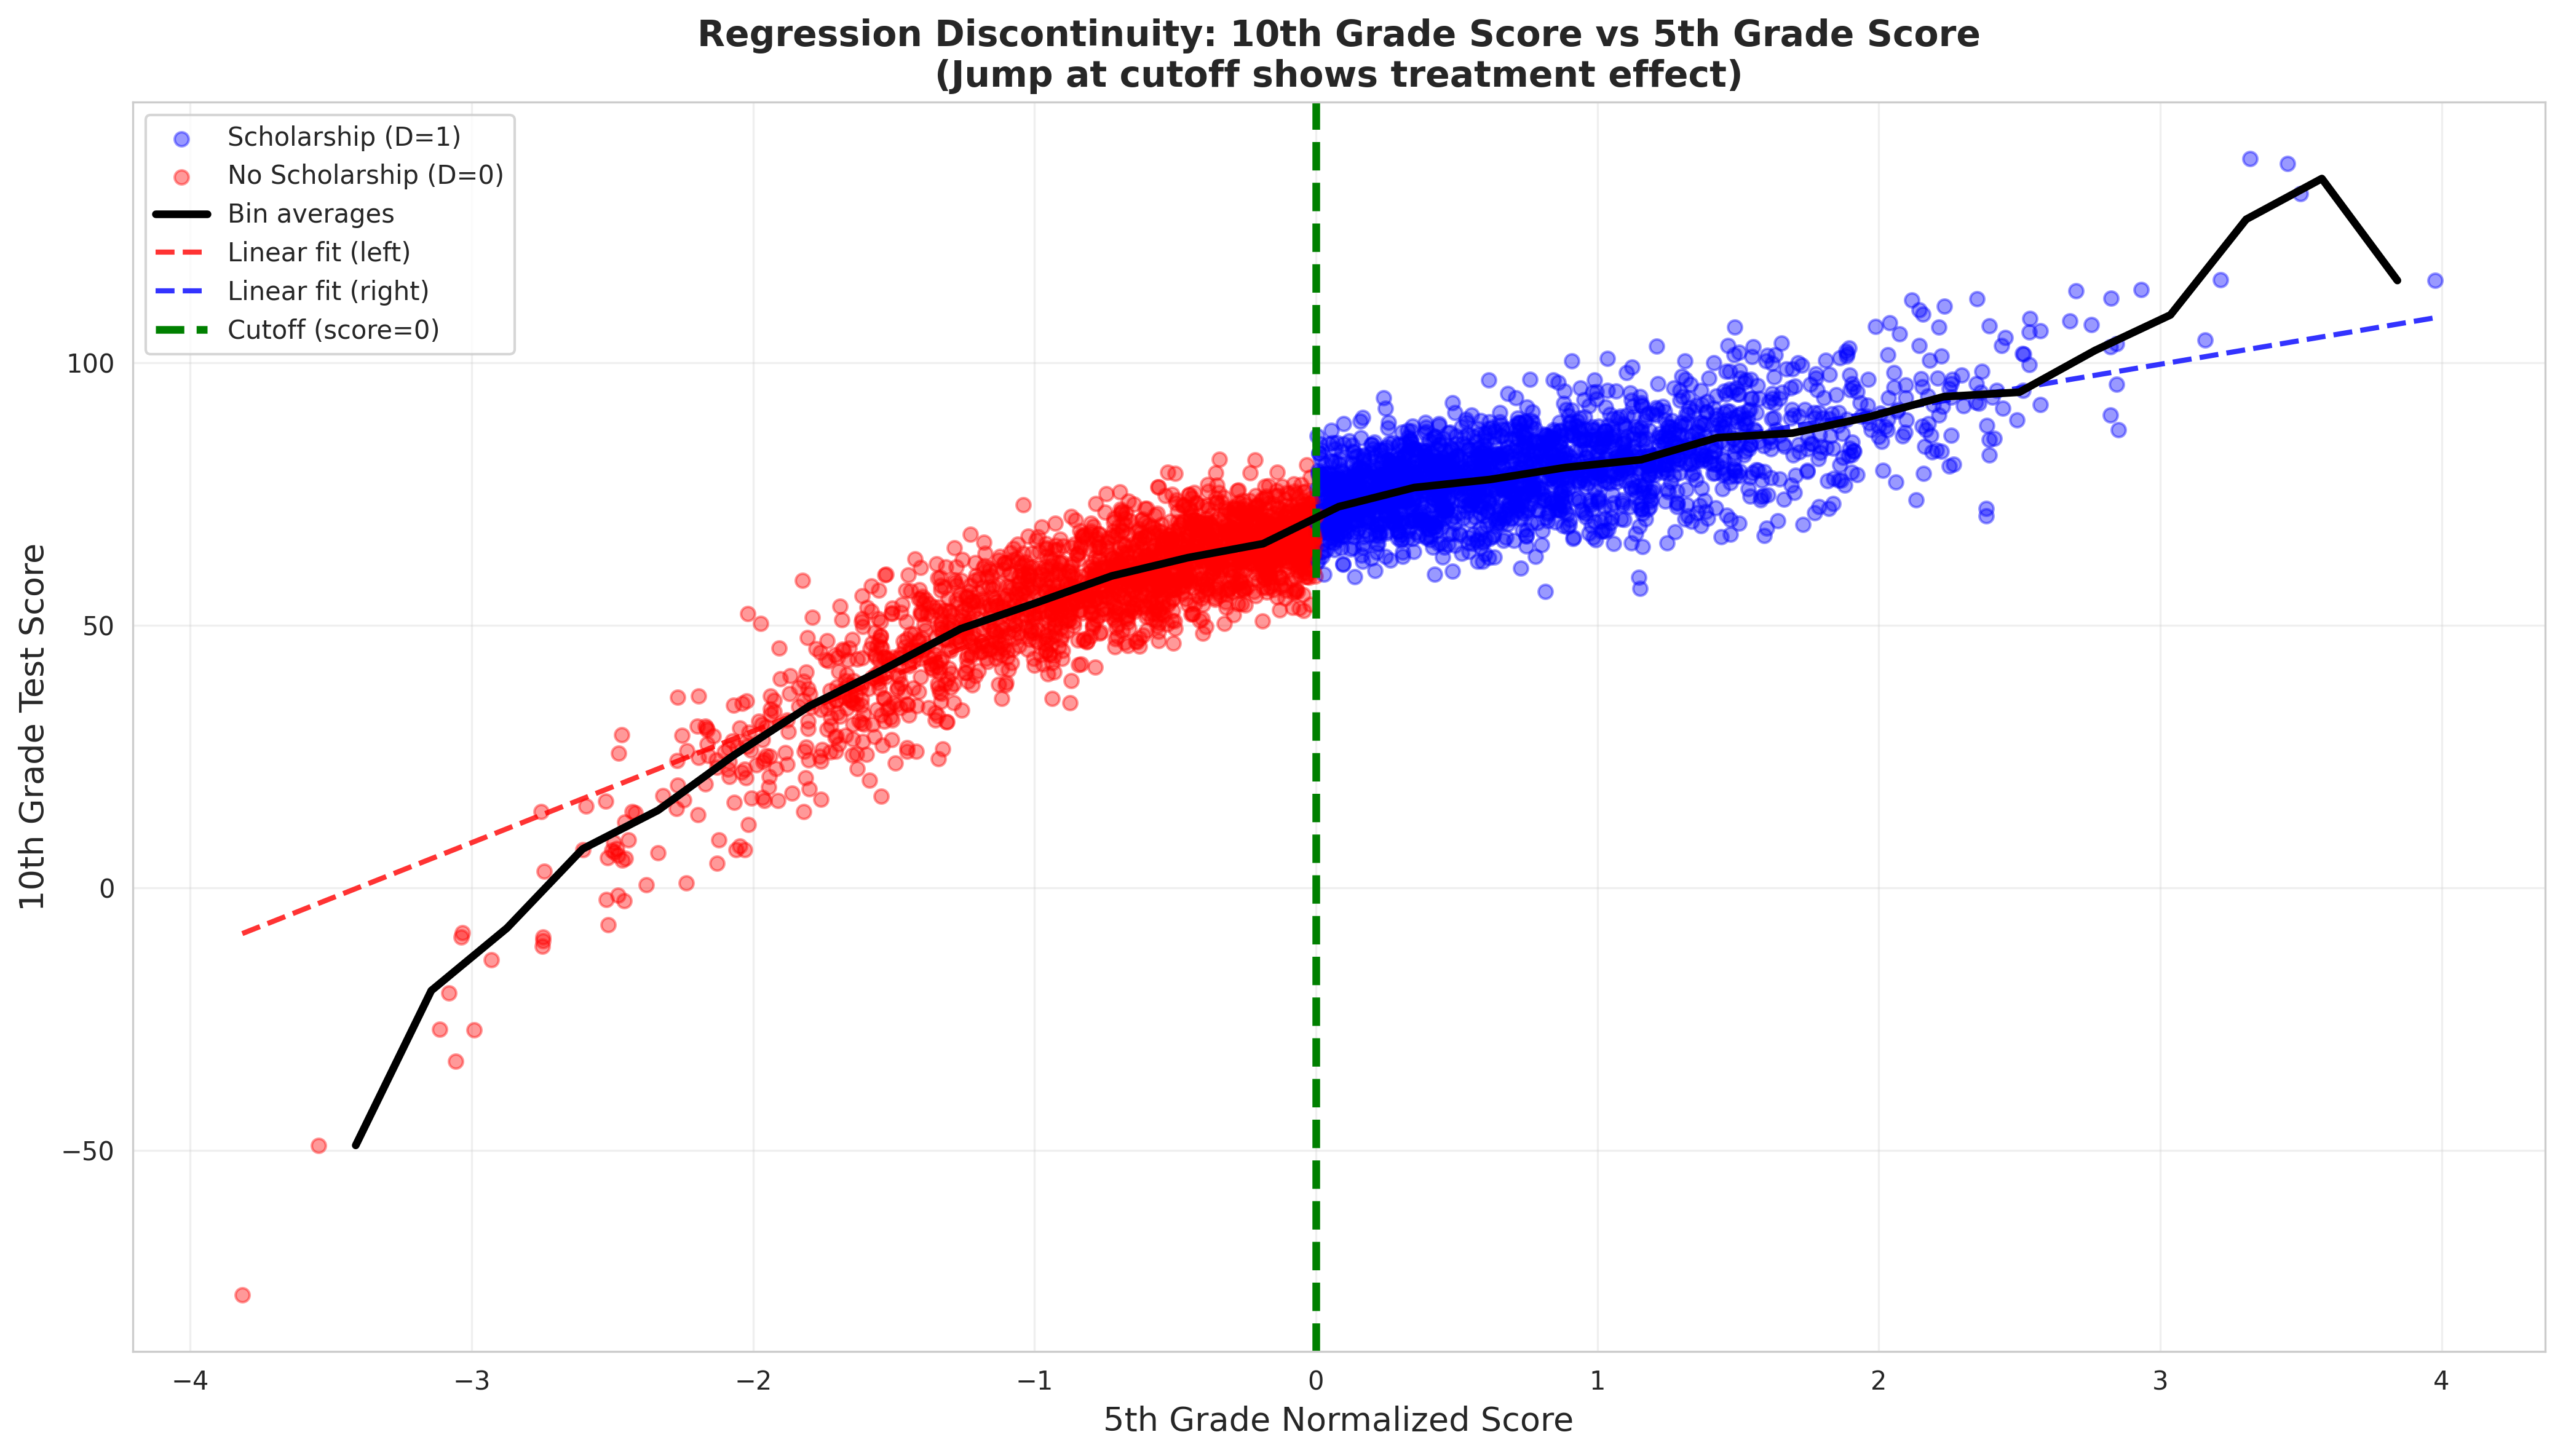
\includegraphics[width=0.9\textwidth]{rdd_discontinuity_plot.png}
    \caption{Regression discontinuity: 10th grade score vs. 5th grade score. Red points represent students without scholarship (D=0), blue points represent scholarship recipients (D=1). The green vertical line marks the cutoff at score = 0.}
    \label{fig:rdd_discontinuity}
\end{figure}

\subsubsection{RDD Estimation Results}

Three models were estimated to assess the scholarship's causal effect:

\begin{table}[H]
\centering
\begin{tabular}{lcccc}
\toprule
Model & Treatment Effect & Std. Error & p-value & R-squared \\
\midrule
Basic RDD & 0.362 & 0.429 & 0.399 & 0.770 \\
RDD with Interaction & 0.188 & 0.384 & 0.624 & 0.816 \\
RDD with Covariates & 0.152 & 0.383 & 0.692 & 0.817 \\
\midrule
Local (bandwidth=0.5) & \textbf{6.131} & 0.546 & <0.001 & -- \\
\bottomrule
\end{tabular}
\caption{RDD estimation results. The full sample shows no significant effect, but local linear regression near the cutoff reveals a large, significant effect.}
\label{tab:rdd_results}
\end{table}

\textbf{Full Model Results (with covariates):}
\begin{itemize}
    \item Treatment effect (τ): 0.152 points
    \item p-value: 0.692 (not significant)
    \item Hours studied: +0.237 points per hour (p < 0.001) ***
    \item Mother's education: +0.045 points per year (p = 0.437)
    \item Female: +0.079 points (p = 0.734)
\end{itemize}

\textbf{Local Linear Regression (robustness check):}
\begin{itemize}
    \item Using bandwidth = 0.5 (1,552 observations near cutoff)
    \item Treatment effect: 6.131 points (p < 0.001)
    \item Highly significant, but very different from full sample estimate
\end{itemize}

\textbf{Interpretation:}
The full sample analysis suggests no statistically significant effect of scholarship on 10th grade scores. However, the local estimate near the cutoff shows a large, significant effect. This discrepancy, combined with evidence of covariate manipulation, suggests:
\begin{enumerate}
    \item The RDD assumptions may be violated
    \item The treatment effect may be heterogeneous along the running variable
    \item Hours studied is a stronger predictor of test scores than scholarship receipt
\end{enumerate}

\section{Discussion}

\subsection{Difference-in-Difference Analysis}

The DiD analysis provides strong evidence that government subsidies have a positive causal effect on regional wages. Key findings include:

\begin{enumerate}
    \item \textbf{Significant Treatment Effect:} The subsidy increases wages by \$1.68--\$1.79 (p < 0.001)
    \item \textbf{Robustness:} Results are stable across specifications (with/without controls)
    \item \textbf{Parallel Trends:} Pre-treatment trends appear reasonably parallel, supporting the identifying assumption
    \item \textbf{Heterogeneity:} Manufacturing experiences the largest benefit, possibly due to sector-specific mechanisms
\end{enumerate}

\textbf{Policy Implications:}
The findings suggest that government subsidies effectively boost regional wages, with manufacturing regions benefiting most. Policymakers could target subsidies to maximize impact across sectors.

\subsection{Regression Discontinuity Design}

The RDD analysis yields mixed results:

\begin{enumerate}
    \item \textbf{No Effect in Full Sample:} Scholarship receipt shows no significant impact (p = 0.692)
    \item \textbf{Large Local Effect:} Near the cutoff, the effect is 6.13 points (p < 0.001)
    \item \textbf{Assumption Violations:} Covariates show discontinuities, suggesting manipulation
    \item \textbf{Hours Studied Matters:} Study time is a stronger predictor than scholarship receipt
\end{enumerate}

\textbf{Caveats:}
The RDD results should be interpreted with caution due to evidence of potential manipulation at the cutoff. The discrepancy between full sample and local estimates warrants further investigation.

\section{Conclusion}

This report demonstrates the application of two powerful causal inference methods to economic data:

\begin{itemize}
    \item \textbf{DiD Analysis:} Successfully identifies a significant positive effect of government subsidies on wages (\$1.68--\$1.79), with heterogeneous impacts across sectors. The parallel trends assumption appears satisfied, lending credibility to the results.
    
    \item \textbf{RDD Analysis:} Reveals no significant scholarship effect in the full sample, but large local effects near the cutoff. Evidence of covariate manipulation suggests caution in interpretation. Hours studied emerges as a key predictor of test scores.
\end{itemize}

Both methods highlight the importance of careful assumption testing and robustness checks in causal inference. The analyses provide actionable insights for policy evaluation in economics.

\subsection{Limitations and Future Work}

\begin{itemize}
    \item \textbf{DiD:} Assumes no spillover effects between treated and control regions
    \item \textbf{RDD:} Potential manipulation at cutoff; local effect may not generalize
    \item \textbf{Future Work:} Event study analysis for DiD; donut-hole RDD to address manipulation
\end{itemize}

\section{Code and Reproducibility}

All analyses were implemented in Python using the following packages:
\begin{itemize}
    \item \texttt{pandas}, \texttt{numpy}: Data manipulation
    \item \texttt{matplotlib}, \texttt{seaborn}: Visualization
    \item \texttt{statsmodels}: Econometric modeling
    \item \texttt{scipy}: Statistical tests
\end{itemize}

The complete code and datasets are available at: \href{https://github.com/introspective321/Sem_7_assignments}{\color{HyperlinkBlue}GitHub Repository}.

To reproduce the analysis:
\begin{lstlisting}[language=bash]
# Install dependencies
pip install -r requirements.txt

# Run both analyses
python main.py

# Or run individually
python did_analysis.py
python rdd_analysis.py
\end{lstlisting}

\end{document}
